% ----------------------------------------------------
% Implementation
% ----------------------------------------------------

\chapter{PCB Construction, Adjustments and Code}

\section{PCB Design}

The circuits for the probe, controller and gold electrode \glspl{pcb} were designed using KiCad and manufactured with \texttt{JLCPCB}.
The gold electrodes was trivial, only requiring a single layer \gls{pcb} with pads and traces.

The probe \gls{pcb} was more complex, fabricated on a 4-layer \gls{pcb} which is shown in \reffig{fig:probe-pcb}.
\texttt{JLCPCB} offered a discount for 4-layer \glspl{pcb} that were less than $50\times 50mm$ in size which what the dimensions of the probe \gls{pcb} were.
While the probe should ideally be as small as possible to fit through the ice core, the probe was not designed smaller than $50\times 50mm$ to allow for an easier debugging process.

%chktex-file 44
\begin{figure}[ht]
    \begin{minipage}{0.5\textwidth}
        \centering
        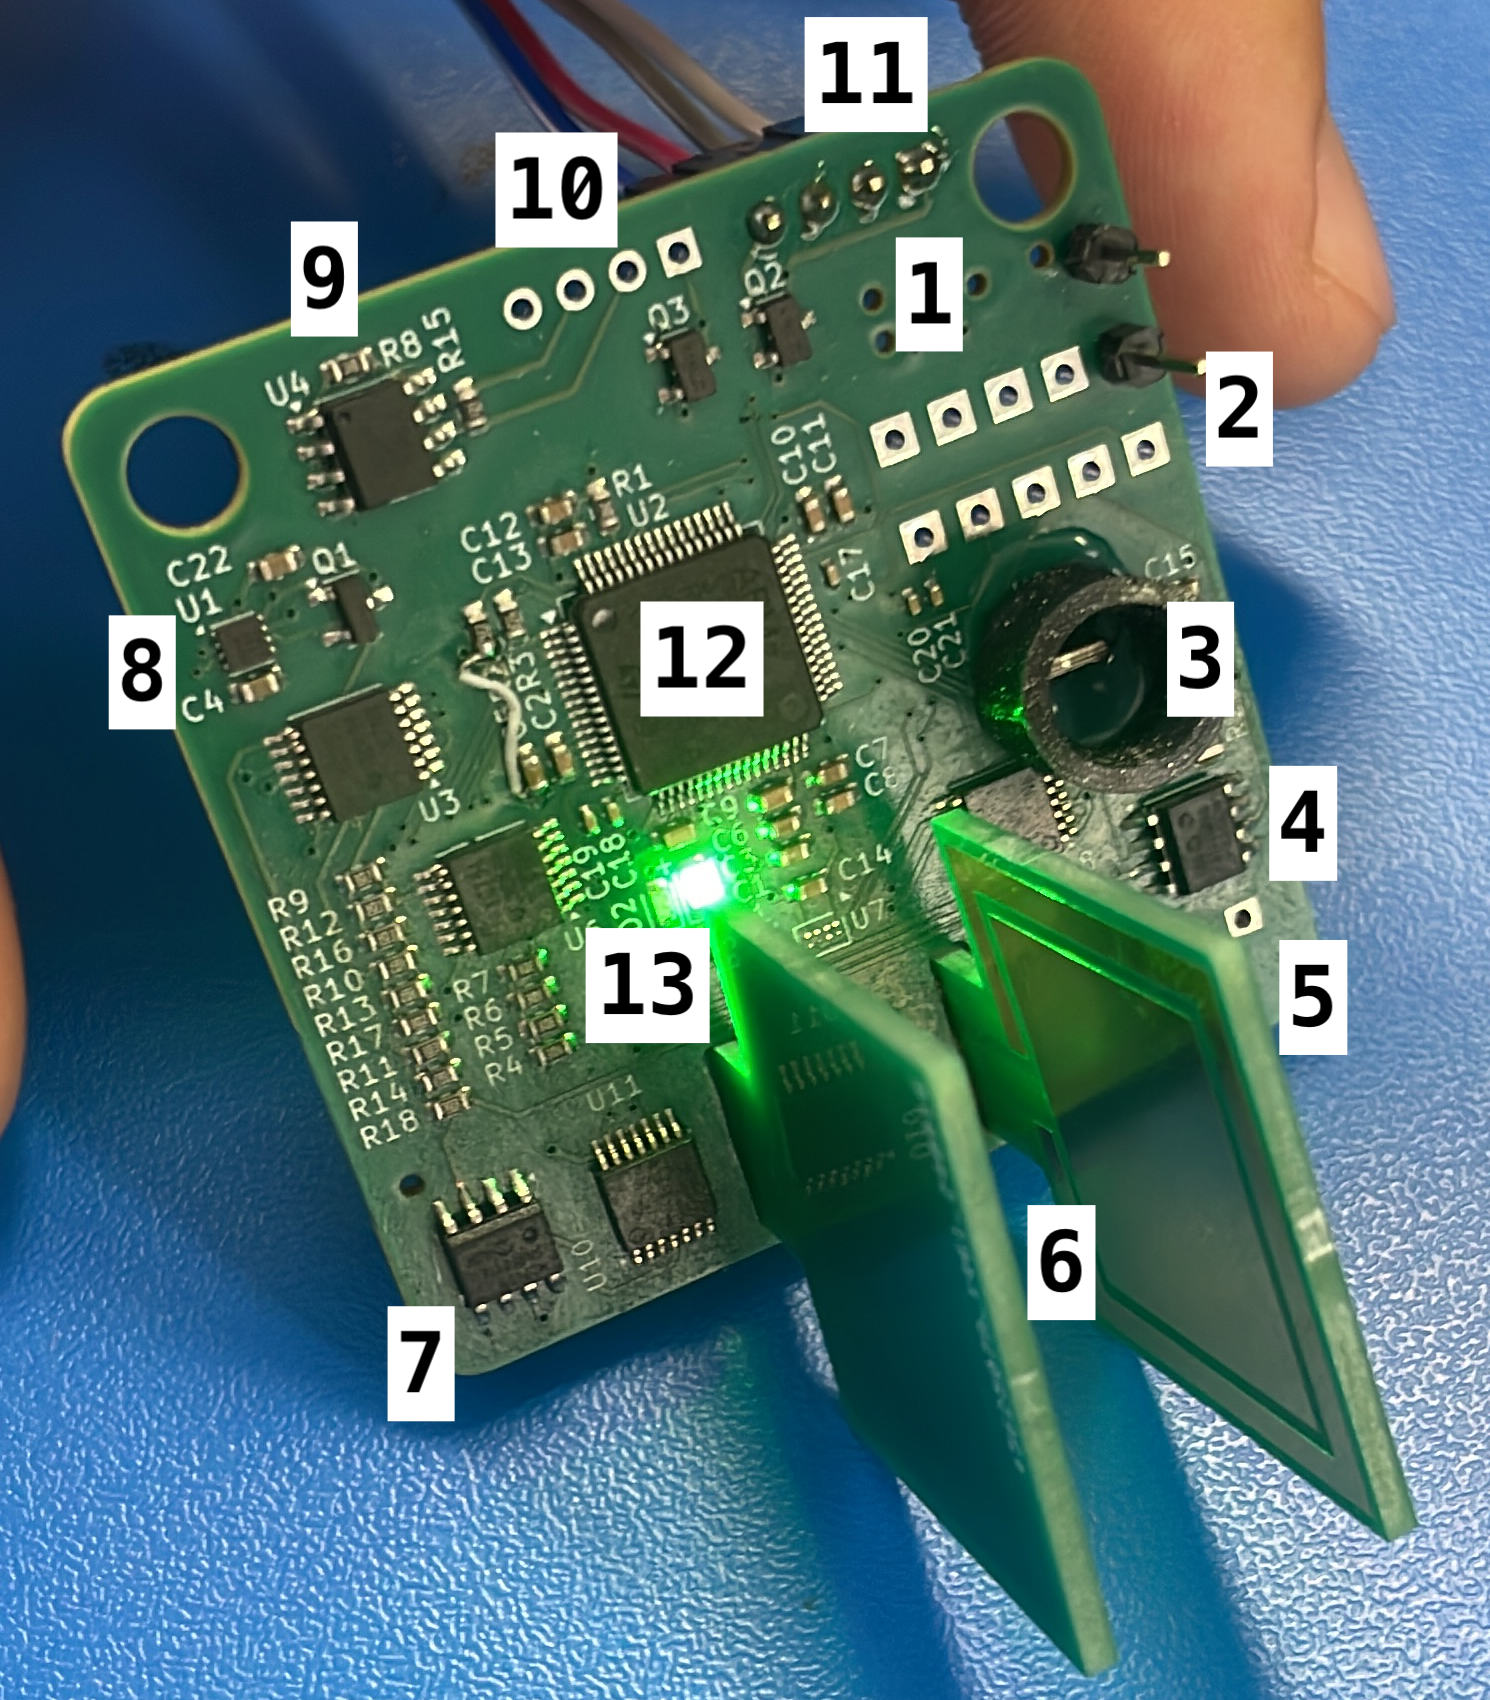
\includegraphics[width=0.8\textwidth]{Figures/probe_pcb}
        \caption{The probe PCB with the gold electrodes attached and adjustments made}
        \label{fig:probe-pcb} %chktex 24
    \end{minipage}
    \begin{minipage}{0.5\textwidth}
        \centering
        \begin{longtblr}[
            caption=\reffig{fig:probe-pcb} Key,
        ]
        {
            hlines,
            colspec = {Q[c,m] Q[l,m,7cm]},
        }
            1 & Programmer Port \\
            2 & Test Points \\
            3 & Pressure Sensor in a Protective Housing \\
            4 & $11\times$ Gain Op-Amp \\
            5 & Titanium Electrode Port \\
            6 & Gold Electrodes \\
            7 & Unity Gain Buffer Op-amp \\
            8 & \gls{dac} and Buffer Transistor \\
            9 & \gls{uart} to \gls{rs485} Converter \\
            10 & \gls{rs485} Port \\
            11 & \gls{uart} Port \\
            12 & STM32F4 Microcontroller \\
            13 & \glspl{led} \\
        \end{longtblr}
    \end{minipage}
    \vspace{0.2cm} \\
    \textit{Note 1: The rest of the titanium electrode ports are behind the gold electrode.} \\
    \textit{Note 2: The other \glspl{ic} present are the TS3A4751 switches.}
\end{figure}

The probe was designed with the resistance measuring circuitry, temperature and pressure sensors, microcontroller, \gls{uart} to \gls{rs485} converter and \gls{rs485} port mentioned in \refch{ch:design}.
The gold and titanium electrodes were given ports at the bottom of the board such that they sat perpendicular to the board which was deemed the easiest method of attachment.
A \gls{uart} port was added next to the \gls{rs485} port to allow for debugging and testing of the probe without the controller.
Both of these ports were also made with reverse polarity protection to prevent unintentional damage to the board. 
Lastly, \glspl{led} were added next to the microcontroller and a programmer port and test points were added at the top of the board to allow for easy debugging and testing of the board.
Having the programmer and communication ports at the top of the board allowed the lower half of it with the probes to be submerged while still being able to communicate with the board.

The controller \gls{pcb} was fabricated on a 2-layer board, which is shown in \reffig{fig:controller-pcb}, as the components were too large to fit on a $50\times 50mm$ 4-layer board.
\texttt{JLCPCB} offered a similar discount for 2-layer \glspl{pcb} that were less than $100\times 100mm$ which is what the dimensions of the controller were restricted to.
Ultimately, the dimensions were made to be $100\times 60mm$ as this area could comfortably fit all the components.

\begin{figure}[ht]
    \begin{minipage}{0.5\textwidth}
        \centering
        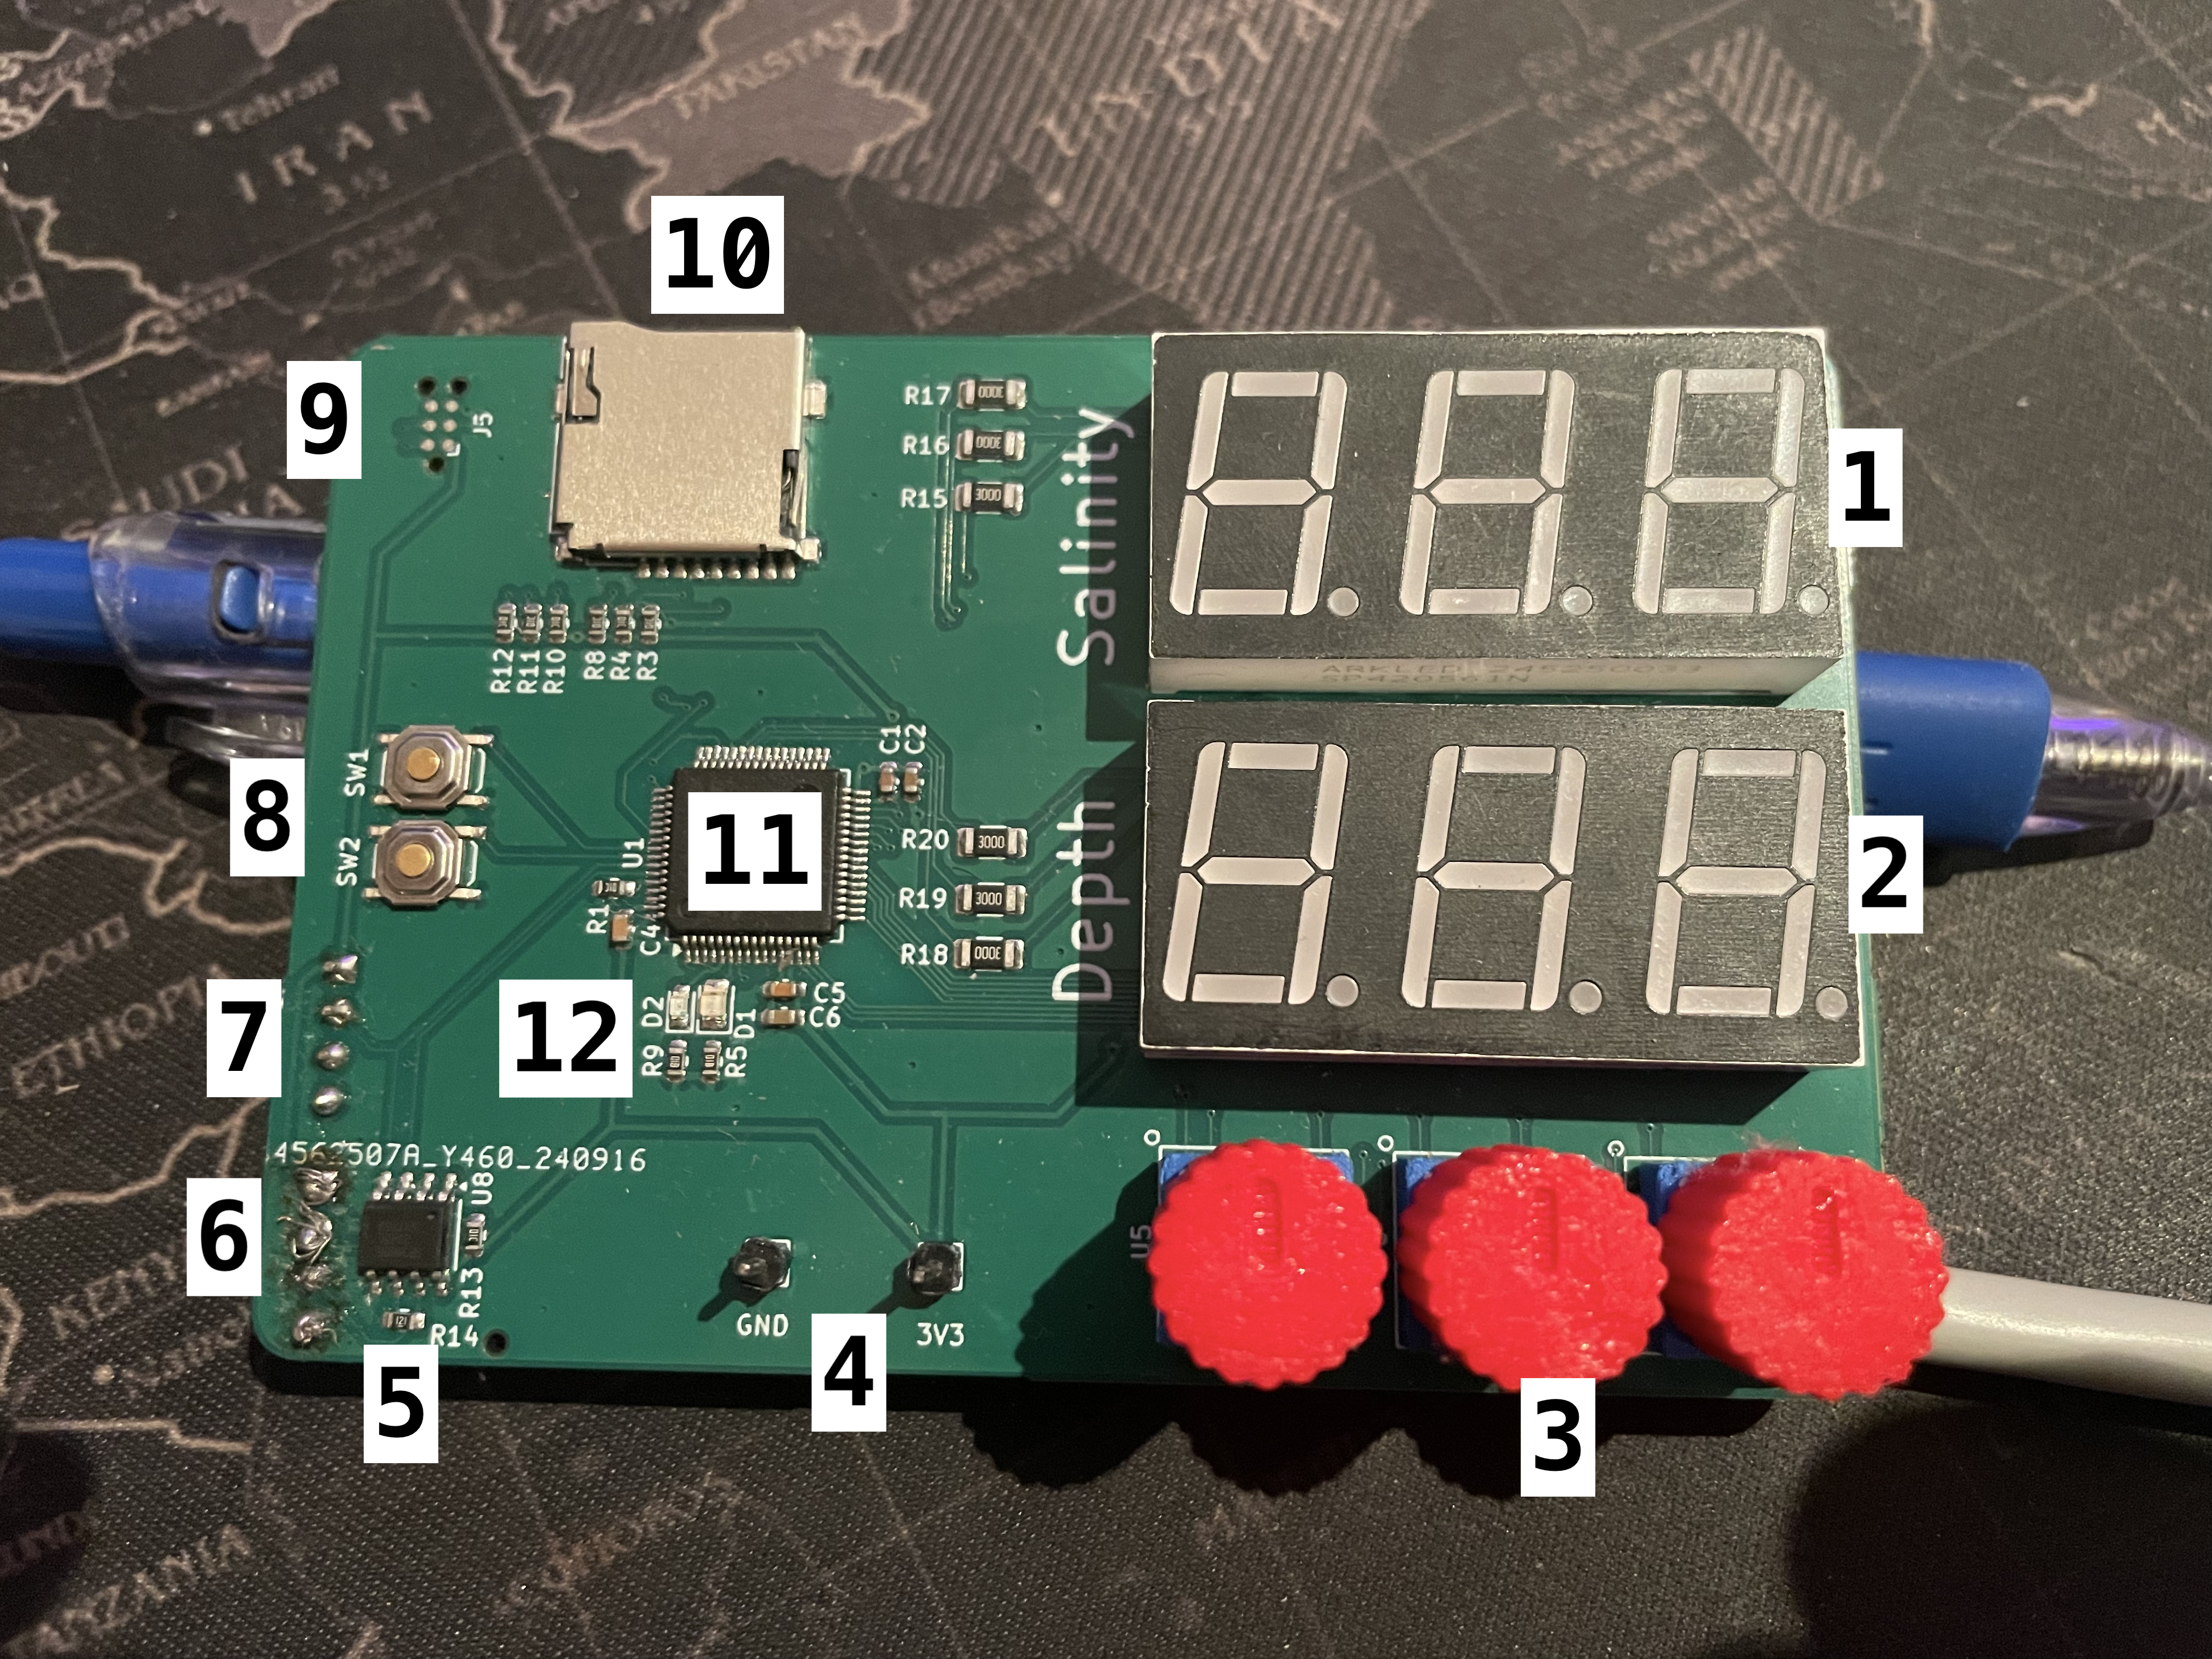
\includegraphics[width=\textwidth]{Figures/controller_pcb_final}
        \caption{The controller PCB with the rotary switch caps attached}
        \label{fig:controller-pcb} %chktex 24
    \end{minipage}
    \begin{minipage}{0.5\textwidth}
        \centering
        \begin{longtblr}[
            caption=Figure Key,
        ]
        {
            hlines,
            colspec = {Q[c,m] Q[l,m]},
        }
            1 & Salinity 7-Segment Display \\
            2 & Depth 7-Segment Display \\
            3 & Rotary Switches \\
            4 & Power Input \\
            5 & \gls{uart} to \gls{rs485} Converter \\
            6 & \gls{rs485} Port \\
            7 & \gls{uart} Port \\
            8 & Input Buttons \\
            9 & Programmer Port \\
            10 & SD Card Port \\
            11 & STM32F0 Microcontroller \\
            12 & \glspl{led} \\
        \end{longtblr}
    \end{minipage}
\end{figure}

The controller was designed with the rotary switches, 7-segment displays, \gls{uart} to \gls{rs485} converter and \gls{rs485} port mentioned in \refch{ch:design}.
The 7-segment displays were designated a default of displaying the salinity and depth of the water using silkscreen, but they could be changed to display anything using software.
The components were placed in a user-friendly manner allowing for easy use of the buttons and rotary switches.
Similarly to the probe, \glspl{led}, a \gls{uart} port and a programmer port added to the board to allow for debugging and testing of the board.
It should be noted that an SD Card Port was added for future expansion but was not used nor tested during this project.

\section{PCB Adjustments}

There were three adjustments made to the probe \gls{pcb} to ensure that it was functioning as expected excluding the soldering of the headers and gold electrodes.
Firstly, one of the pins of the microcontroller was incorrectly not connected to power and was corrected by soldering a wire to connect it to power which can be seen of the left of the microcontroller.
Secondly, the footprint of the pressure sensor was incorrectly flipped horizontally which was corrected by flipping and soldering the depth sensor vertically.
A protective case was added around the pressure sensor to prevent it from being damaged during testing and the casing would also later function as the support for the waterproof membrane that would create the pressure seal.

Lastly, both op-amps were incorrectly chosen and thus had to be replaced with new op-amps that shared the same footprint.
The temperature sensor also had an incorrect footprint, but this was not able to be rectified as this was discovered after the board had already been manufactured, and thus the temperature sensor was not soldered to the board.
The pressure sensor's onboard temperature sensor was used instead.

The controller \gls{pcb} required no adjustments as the design was simple, and the components were all correctly placed.
There was one minor error with pin assignments with the rotary switch pins, but this was corrected in software and did not require any hardware changes.
Switch caps for the rotary switches were 3D printed and attached to the shafts of the rotary switches to make them easier to turn and to make the controller more user-friendly.
It should be noted that the SD Card Port was added for future expansion and was not used nor tested during this project.

\section{Probe Code}

The major steps in measuring salinity are to measure the conductivity of the water between the electrodes, measure the temperature and pressure of the water and then calculate the salinity.
An overview of this process along with the process for each major measurement is shown in \reffig{fig:probe-code-flowchart}.

\begin{figure}[ht]
    \centering
    \includegraphics[width=1\textwidth]{Figures/probe_flowchart}
    \caption{The flowchart for the probe code that measures salinity.}
    \label{fig:probe-code-flowchart} %chktex 24
\end{figure}

The conductivity measurement and calculation is different depending on if the voltage-resistance relationship is constant or not which is expected for the gold and titanium electrodes respectively.
Both variations start with a voltage sweep where the voltage is increased from the minimum to the maximum voltage with a set voltage step or vice versa by the \gls{dac}.
At each step, the voltage output of the \gls{dac}, the voltage across the calibration resistor and the voltage across the electrodes are measured.

If the ratio between the \gls{dac} voltage and the voltage across the electrodes is not constant, the conductivity will have to be determined by performing tests to create a model that can relate a set voltage samples to a conductivity. 

If the ratio between the \gls{dac} voltage and the voltage across the electrodes is constant, the resistance between the electrodes can be calculated using the calibration resistor.
Given that the calibration resistance and $R_1$ is known, the resistance between the electrodes can be calculated for each voltage sample using the ratio between the electrode and calibration voltages as shown in \refeqn{eqn:electrode-calib-resistance}.
$k$ is calculated using the known values $V_{ratio}$, $R_1$ and $R_{calibration}$ to simplify the equation as shown in \refeqn{eqn:electrode-calib-resistance-simplified} and finally $R_{electrode}$ can be calculated using \refeqn{eqn:electrode-calib-resistance-final}.
\begin{align}
    V_{ratio} &= \lfrac{V_{DAC}A_{11}A_{ADC}\lfrac{R_{electrode}}{R_1 + R_{electrode}}}{V_{DAC}A_{11}A_{ADC}\lfrac{R_{calibration}}{R_1 + R_{calibration}}} = \lfrac{\lfrac{R_{electrode}}{R_1 + R_{electrode}}}{\lfrac{R_{calibration}}{R_1 + R_{calibration}}} \label{eqn:electrode-calib-resistance} \\
    \lfrac{R_{electrode}}{R_1 + R_{electrode}} &= V_{ratio} \lfrac{R_{calibration}}{R_1 + R_{calibration}} = k \label{eqn:electrode-calib-resistance-simplified} \\
    R_{electrode} &= \lfrac{kR_1}{1 - k} \label{eqn:electrode-calib-resistance-final}
\end{align}
The resistance can then be averaged and the conductivity can be calculated for the gold electrodes using \refeqn{eqn:conductivity-from-resistance}.
Using this method allows for the device to nullify all scalar inaccuracies in the circuit including $R_1$ uncertainty, \gls{dac} and \gls{adc} gain errors, and the op-amp gain error as they will all be present in the calibration resistor and the electrodes measurements.
This method is however still vulnerable to offset inaccuracies including \gls{dac} and \gls{adc} offset errors and the internal resistance of the switches and traces.

Measuring the temperature and pressure is a simple matter of reading the temperature sensor and the pressure sensor respectively which finally allows salinity to be calculated which can be performed on the salinometer microcontroller as it possesses an \gls{fpu}.
Additionally, any of the temperature, depth, resistance or conductivity measurements can be calculated individually and transmitted to the controller if requested.

\section{Controller Code}

For the prospective user, the controller's primary function is to instruct the probe to take a measurement and then to display said measurement, but for the purpose of testing and investigation, the controller was given additional functionality.
The main functions of the controller are to instruct the probe to take a measurement, to display the measurement, and to allow for configuration of the probe.

The display was done using 7-segment displays to display the various measurements.
Each digit of the 7-segment display was written to by writing the 7-segment digit code and keeping the corresponding digit's cathode low while keeping the others high.
This was repeated for each digit in quick succession using timer controlled \gls{dma} to give the illusion of all digits being on at the same time.

The left most rotary switch was used to navigate the menu.
The menu included the default of showing both salinity and depth, showing individual measurements of temperature, depth, resistance, conductivity and salinity, and the configurable parameters of the probe.
The menu names were displayed on the top row of the 7-segment display and the selected menu item was displayed on the bottom row.
This created some limitations on what could be displayed, for instance the best display of temperature was `teP', but all menu items were still reasonably clear.

When the user selected a measurement menu item, the top switch was configured to request that measurement from the probe and display it and when the user selected the configuration menu item, the top switch was configured to update the probe's configuration.
The other two rotary switches were used to adjust the configurable parameters of the probe which are discussed further in \refsec{sec:board-to-board-communication}.
The bottom switch was configured to reset the probe and the controller should an error occur.

\section{Board to Board Communication}\label{sec:board-to-board-communication}

The probe and controller communicate using half-duplex \gls{rs485} communication which is buffered on both sides by the \gls{uart} to \gls{rs485} converter.
This makes the protocol effectively half-duplex \gls{uart} communication from the perspective of the microcontrollers.
The probe was configured to be in receive mode where it would be perpetually waiting for a 1 byte command from the controller.
All the possible commands and expected responses are shown in \reffig{fig:rs485-flowchart}.

\begin{figure}[ht]
    \centering
    \includegraphics[width=0.5\textwidth]{Figures/rs485_flowchart}
    \caption{The flowchart for the controller code that communicates with the probe.}
    \label{fig:rs485-flowchart} %chktex 24
\end{figure}

While not directly available to the user, the controller can request a status byte to which the probe will respond with \textit{idle}, \textit{busy} or \textit{error} depending on the state of the probe.
This allows for some simple error checking and communication flow which could be integrated into more robust error handling in the future.
When the user requests a measurement, the controller sends the corresponding request command to which the probe will respond with the measurement data.

When the user requests a configuration update, the controller transfers a configuration packet through the predefined manner shown in \reffig{fig:rs485-flowchart}.
Once the probe is fully cast in epoxy resin, the configuration can only be updated this way so all possibly useful, configurable parameters were included in the configuration packet.
This includes which electrode to use (including whether to use the fringe shield or not), the $R_1$ resistor to use, the directionality of the resistance measurement (unidirectional or bidirectional), the voltage sweep start, end and number of steps among other parameters.
Some parameters such as the directionality are unlikely to be changed from there default value (bidirectional) but were included to cover any unforeseen circumstances.

When the user resets the boards using the bottom switch of the controller, the controller first sends a reset command to the probe before resetting itself.
This command allows for remotely resetting the probe should a system error occur on it, however this only works provided the \gls{rs485} connection is still operational.
Otherwise, the entire system will need to be powered off and on again to reset the probe.
The reset on both microcontroller is triggered using software to setting the \gls{sys_reset_req} bit in the \gls{scb} register which triggers a system reset similar to that of pulling the reset pin low.